\documentclass[a4paper,10pt]{scrartcl}
\usepackage[utf8]{inputenc}
\usepackage[T1]{fontenc}
\usepackage{booktabs}
\usepackage{import}
\usepackage{xspace}
\usepackage{enumitem}
\usepackage{cite}
\usepackage{graphicx}
\usepackage{tikz}
\usepackage{wrapfig}
\usepackage{tikz-uml}
\usepackage{gantt}
\usepackage{pdflscape}
\usetikzlibrary{arrows}
\usetikzlibrary{fit}
\usetikzlibrary{calc}
\usepackage{float}
\usepackage{amssymb}
\usepackage{listings}
\usepackage[section]{placeins} % don't move figures beyond the next section heading

% this is needed for forms and links within the text
\usepackage{hyperref}

% Variables
\newcommand{\authorName}{
   Mohammed~Abu~Jayyab,
   Niklas~Baumstark,
   Tobias~Gräf,
   Amrei~Loose,
   Christoph~Michel
}
\newcommand{\authorNameEmph}{
   Mohammed~Abu~Jayyab,
   Niklas~Baumstark,
   \textbf{Tobias~Gräf},
   Amrei~Loose,
   Christoph~Michel
}

\newcommand{\dateFirstVersion}{\today}
\newcommand{\customer}{Karlsruhe Institute of Technology}
\newcommand{\contractor}{A company}
\newcommand{\projectName}{Broadcast Encryption\xspace}

\newcommand{\doctitle}{\projectName (Design document)}
\title{\doctitle}
\author{\authorName}
\date{\today}

% less margin
\usepackage[margin=2.5cm]{geometry}

% horizontal line
\newcommand{\HRule}{\rule{\linewidth}{0.5mm}}

% more beautiful lists
\setlist{noitemsep}
\renewcommand{\labelitemi}{$\bullet$}
\renewcommand{\labelitemii}{$\diamond$}

% create a shorter version for tables
\newcommand\addrow[2]{#1 &#2\\ }
\newcommand\addheading[2]{\textbf{\sffamily #1} &\textbf{\sffamily #2}\\ \hline}
\newcommand\tabularhead{\begin{tabular}{lp{13cm}}
\hline
}

\newcommand\addmulrow[2]{ \begin{minipage}[t][][t]{2.5cm}#1\end{minipage}%
   &\begin{minipage}[t][][t]{8cm}
    \begin{enumerate} #2   \end{enumerate}
    \end{minipage}\\ }

\newenvironment{usecase}{\tabularhead}
{\hline\end{tabular}}

% a cross
\newcommand\X{$\times$}

% templates and default styles for figures and graphics
\tikzset{>=triangle 45}
\tikzset{font=\sffamily}

\newcommand{\tmpCaption}{}
\newenvironment{illustration}[1]
{
   \renewcommand{\tmpCaption}{#1}
   \begin{figure}[h!]
   \centering
}
{
   \caption{\tmpCaption}
   \end{figure}
}


\begin{document}

\maketitle
  \begin{tabular}[t]{ll}
	Projekt:       & \quad \projektName \\[1.2ex]
	Auftraggeber:  & \quad \auftraggeber\\[1.2ex]
	Auftragnehmer: & \quad \auftragnehmer\\[1.2ex]
  \end{tabular}

\begin{tabular}{|p{3 cm}|p{3 cm}|p{5 cm}|}
\hline
\textbf{Version} & \textbf{Datum} & \textbf{Autor(en)} \\
\hline
\hline
1.0 & 29.04.2012 & \authorName \\
\hline
\end{tabular}

\tableofcontents
\clearpage

\section{Introduction}
In this project we design and implement a software calles Cryptocas. CryptoCast is a piece of software that provides a service to
send contents from a central server to a given group of recipients. Transmission happens via a unidirectional communication channel.
The traffic duplication that would be required for commonly used transport protocols is therefore avoided.

The software enables access control through a specific form of encryption that is based on the Naor-Pinkas broadcast
encryption scheme~\cite[Section~2.2]{Naor00}. The advantage of this scheme is that the communication overhead necessary for session key
management and client revocation does not depend on the total number of recipients, but only on the
number of revoked users.

The type of data that can be transmitted is not determined by the software, so it can be used for a lot
of different sorts of distribution. For demonstration purposes we will implement a simple audio or video
stream.

The server will be realized as a console application and will be able to register new users and revoke
specific users if they are not allowed to receive the stream anymore.

As for the client, it will be realized as an application targetting the Android operating system for smart phones.
It will be able to receive, decode and display the data stream.

We will use a transport protocol based on TCP for the communication between the server and its clients,
but this implementation can easily be replaced by any other protocol that supports reliable, unidirectional
streams (like reliable IP multicast).

Since a broadcast encryption scheme is used, an important goal is to extract the common interface between our
reference implementation of the Naor-Pinkas algorithm and other, similar broadcast encryption schemes.
This way, a more efficient scheme might be used in the future.

In conclusion, our design efforts are focused on modularity and loose coupling between the components of the
infrastructure, so that parts of the program can be exchanged with a minimal amount of necessary changes.

\section{Structure}
\subsection{Architecture}

We implement a client/server model with one central server sending the stream and multiple clients
receiving it.

\begin{illustration}{An overview of all packages.}

\tikzset{
  rect/.style={draw,fill=green!15,minimum height=0.8cm,rectangle},
  box/.style={
    draw=blue!50!white,
    line width=1pt,
    dash pattern=on 1pt off 4pt on 6pt off 4pt,
    inner sep=4mm, rectangle, rounded corners
  },
}

\begin{tikzpicture}[auto,node distance=1.5cm]

\node[rect,minimum width=3cm](util) {cryptocast.util};
\node[rect,minimum width=2cm, xshift=3cm, right of=util](comm) {cryptocast.comm};
\node[rect,minimum width=3cm,xshift=3cm, right of=comm](crypto) {cryptocast.crypto};
\node[rect,minimum width=3cm, xshift=3cm, right of=crypto](naor) {cryptocast.crypto.naorpinkas};
\node[rect,minimum width=3cm, yshift=-2cm, below of=comm](server) {cryptocast.server};
\node[rect,minimum width=3cm, xshift=3cm, right of=server](client) {cryptocast.client};
\node[rect,minimum width=3cm, xshift=3cm, right of=client](file) {cryptocast.client.filechooser};



\draw [<-] (util.south east) -- ( server.north west)
             node[pos=.5]{uses};

\draw [->] (server.north east) -- (crypto.south west);
\draw [->] (server.north east) -- (naor.south west);
\draw [->] (server.north) -- (comm.south);

\draw [->] (crypto.west) -- (comm.east);
\draw [<-] (crypto.east) -- (naor.west);
\draw [->] (client.north east) -- (naor.south west);
\draw [->] (client.north) -- (crypto.south);
\draw [->] (client.north west) -- (comm.south east);

\draw [->] (client.east) -- (file.west);
\end{tikzpicture}

\end{illustration}

Both, server and client, will be based on a three layer architecture to seperate presentation, logic
and storage of the data.
In the case of the server, presentation is handled by the \lstinline|Shell| class, logic is
performed by the \lstinline|Controller|, which in turn uses the \lstinline|ServerData| class
as a data backend.
The client will use the standard MVC model provided by the Android framework.

\begin{illustration}{3-tier architecture of the server}

\tikzset{
  rect/.style={draw,fill=green!15,minimum height=0.8cm,rectangle},
  box/.style={
    draw=blue!50!white,
    line width=1pt,
    dash pattern=on 1pt off 4pt on 6pt off 4pt,
    inner sep=4mm, rectangle, rounded corners
  },
}

\begin{tikzpicture}[auto,node distance=1.5cm]

\node[rect,minimum width=6cm](shell) {\textbf{Shell}};
\node[rect,minimum width=3cm,xshift=-1.5cm,below of=shell](control) {Controller};;
\node[rect,minimum width=3cm,below of=control](data) {ServerData};
\node[rect,minimum width=2cm,xshift=2cm, right of=data](cmd) {Command};

\draw [<->]  (shell.south) --  (control.north)
;
\draw [->]  (shell.south) --  (cmd.north)
  ;
\draw [->]  (control.south) --  (data.north)
  ;

\end{tikzpicture}

\end{illustration}

\section{Package description}

\subimport{../docs/}{cryptocast.comm.tex}
\subimport{../docs/}{cryptocast.crypto.tex}
\subimport{../docs/}{cryptocast.crypto.naorpinkas.tex}
\subimport{../docs/}{cryptocast.util.tex}
\subimport{../docs/}{cryptocast.server.tex}
\subimport{../docs/}{cryptocast.client.tex}
\subimport{../docs/}{cryptocast.client.filechooser.tex}

\section{Sequences}
\begin{illustration}{Server: A command performed in the shell.}
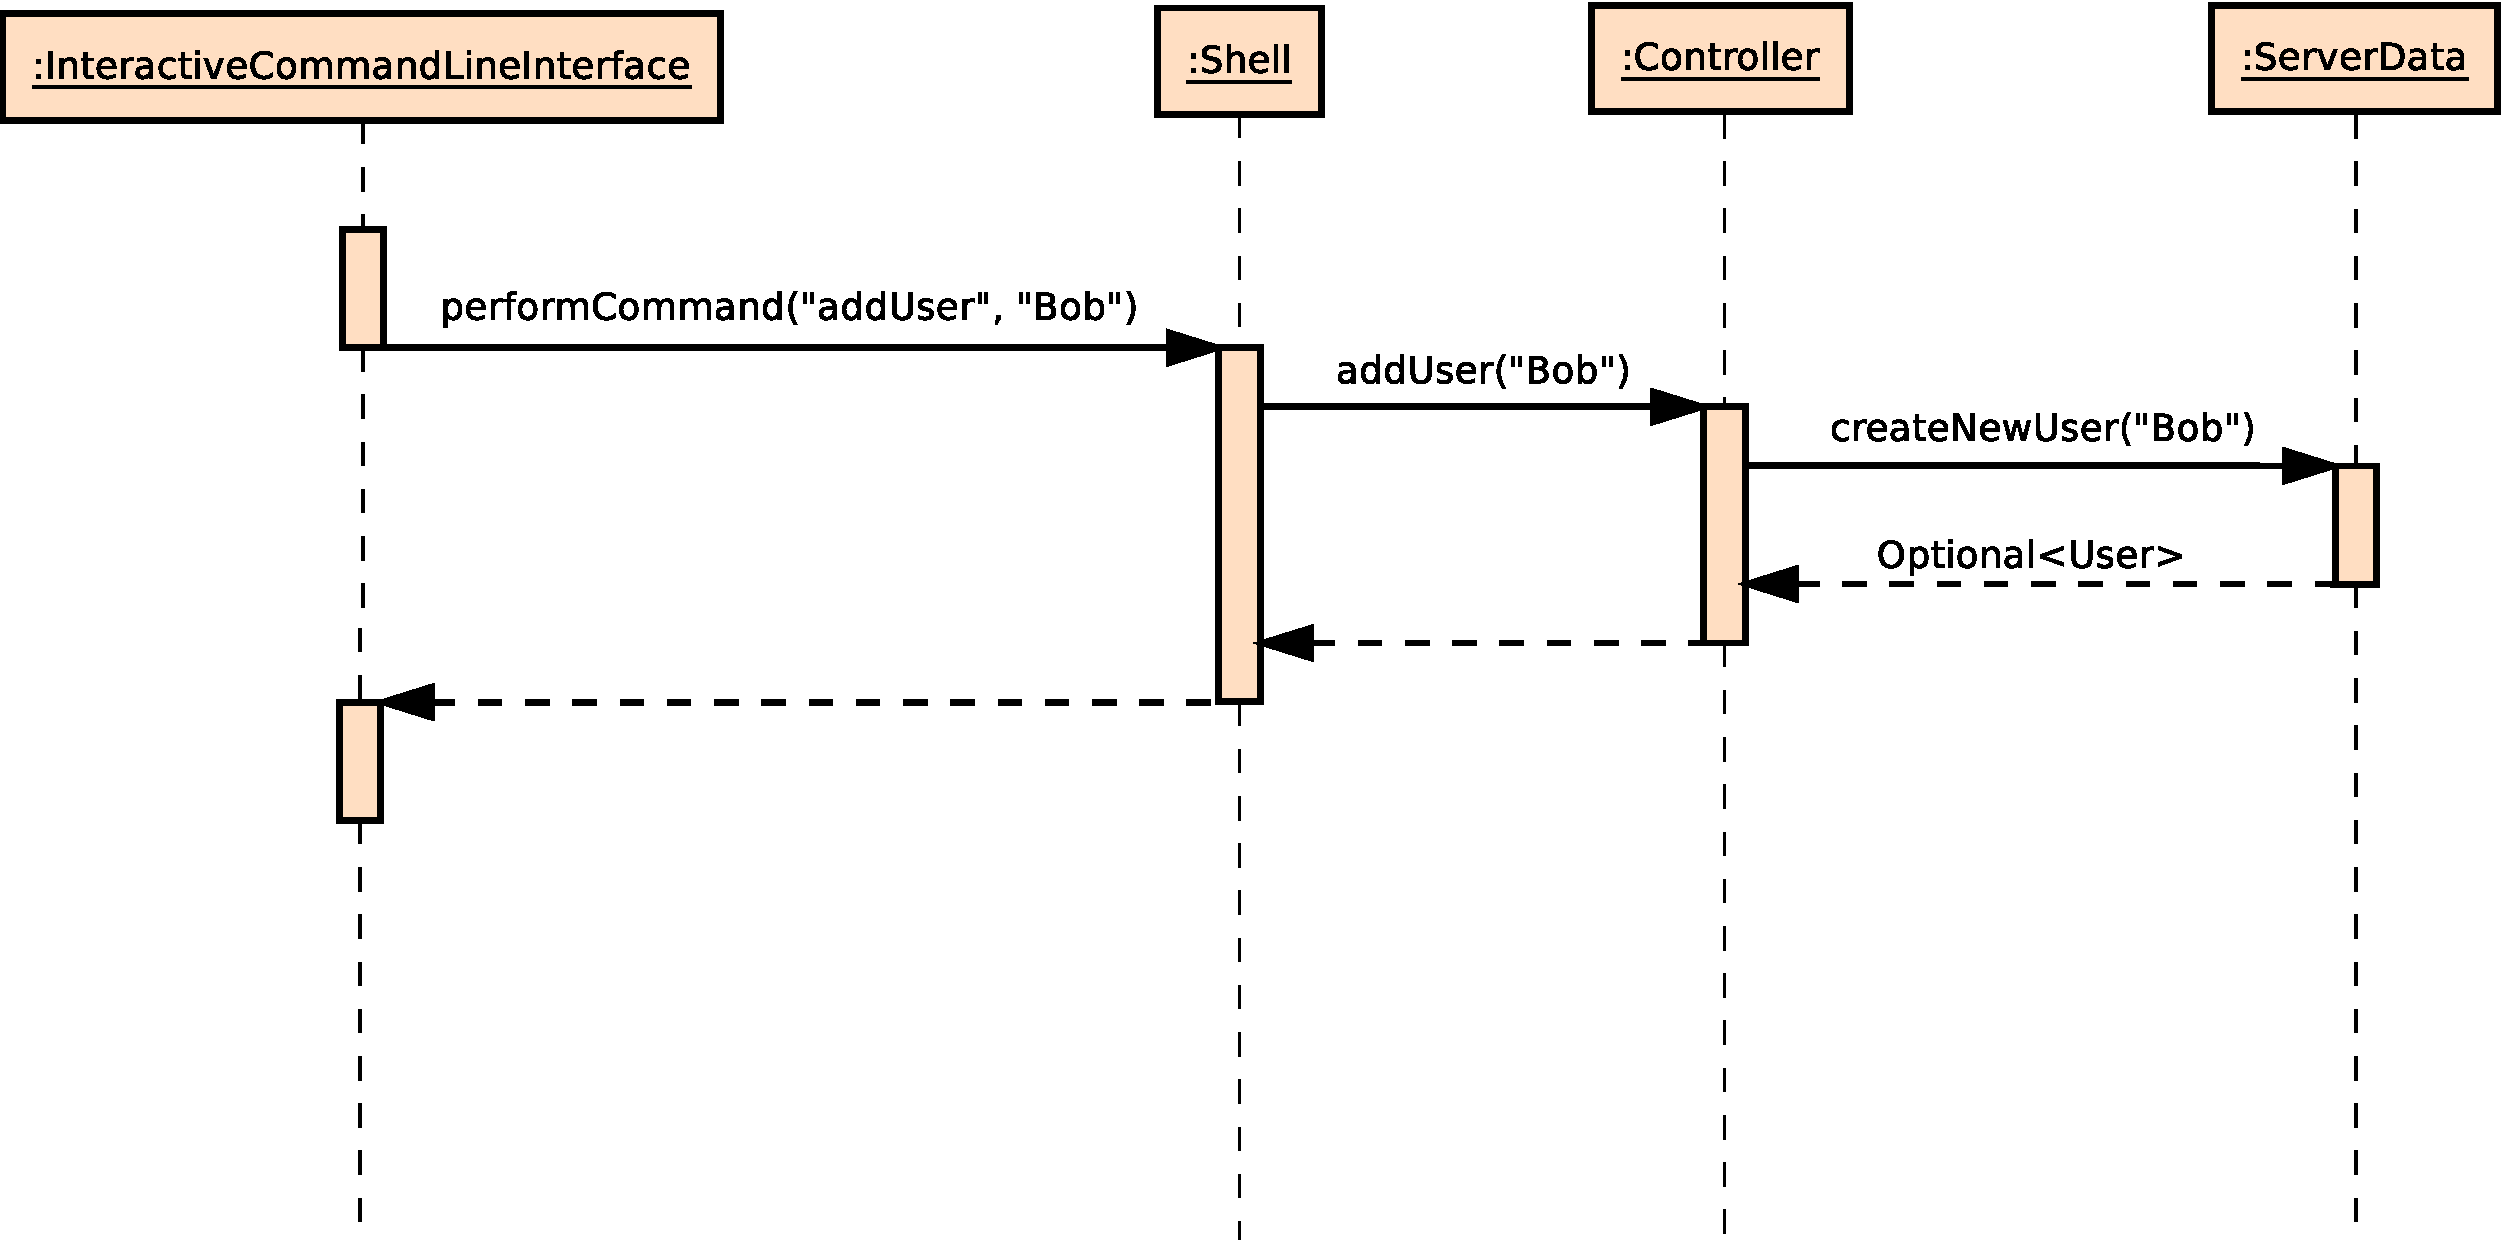
\includegraphics [width=400px] {figures/sequence_diagram_server/Server1.pdf}
\end{illustration}
\begin{illustration}{Client: Connecting to a server for the first time.}
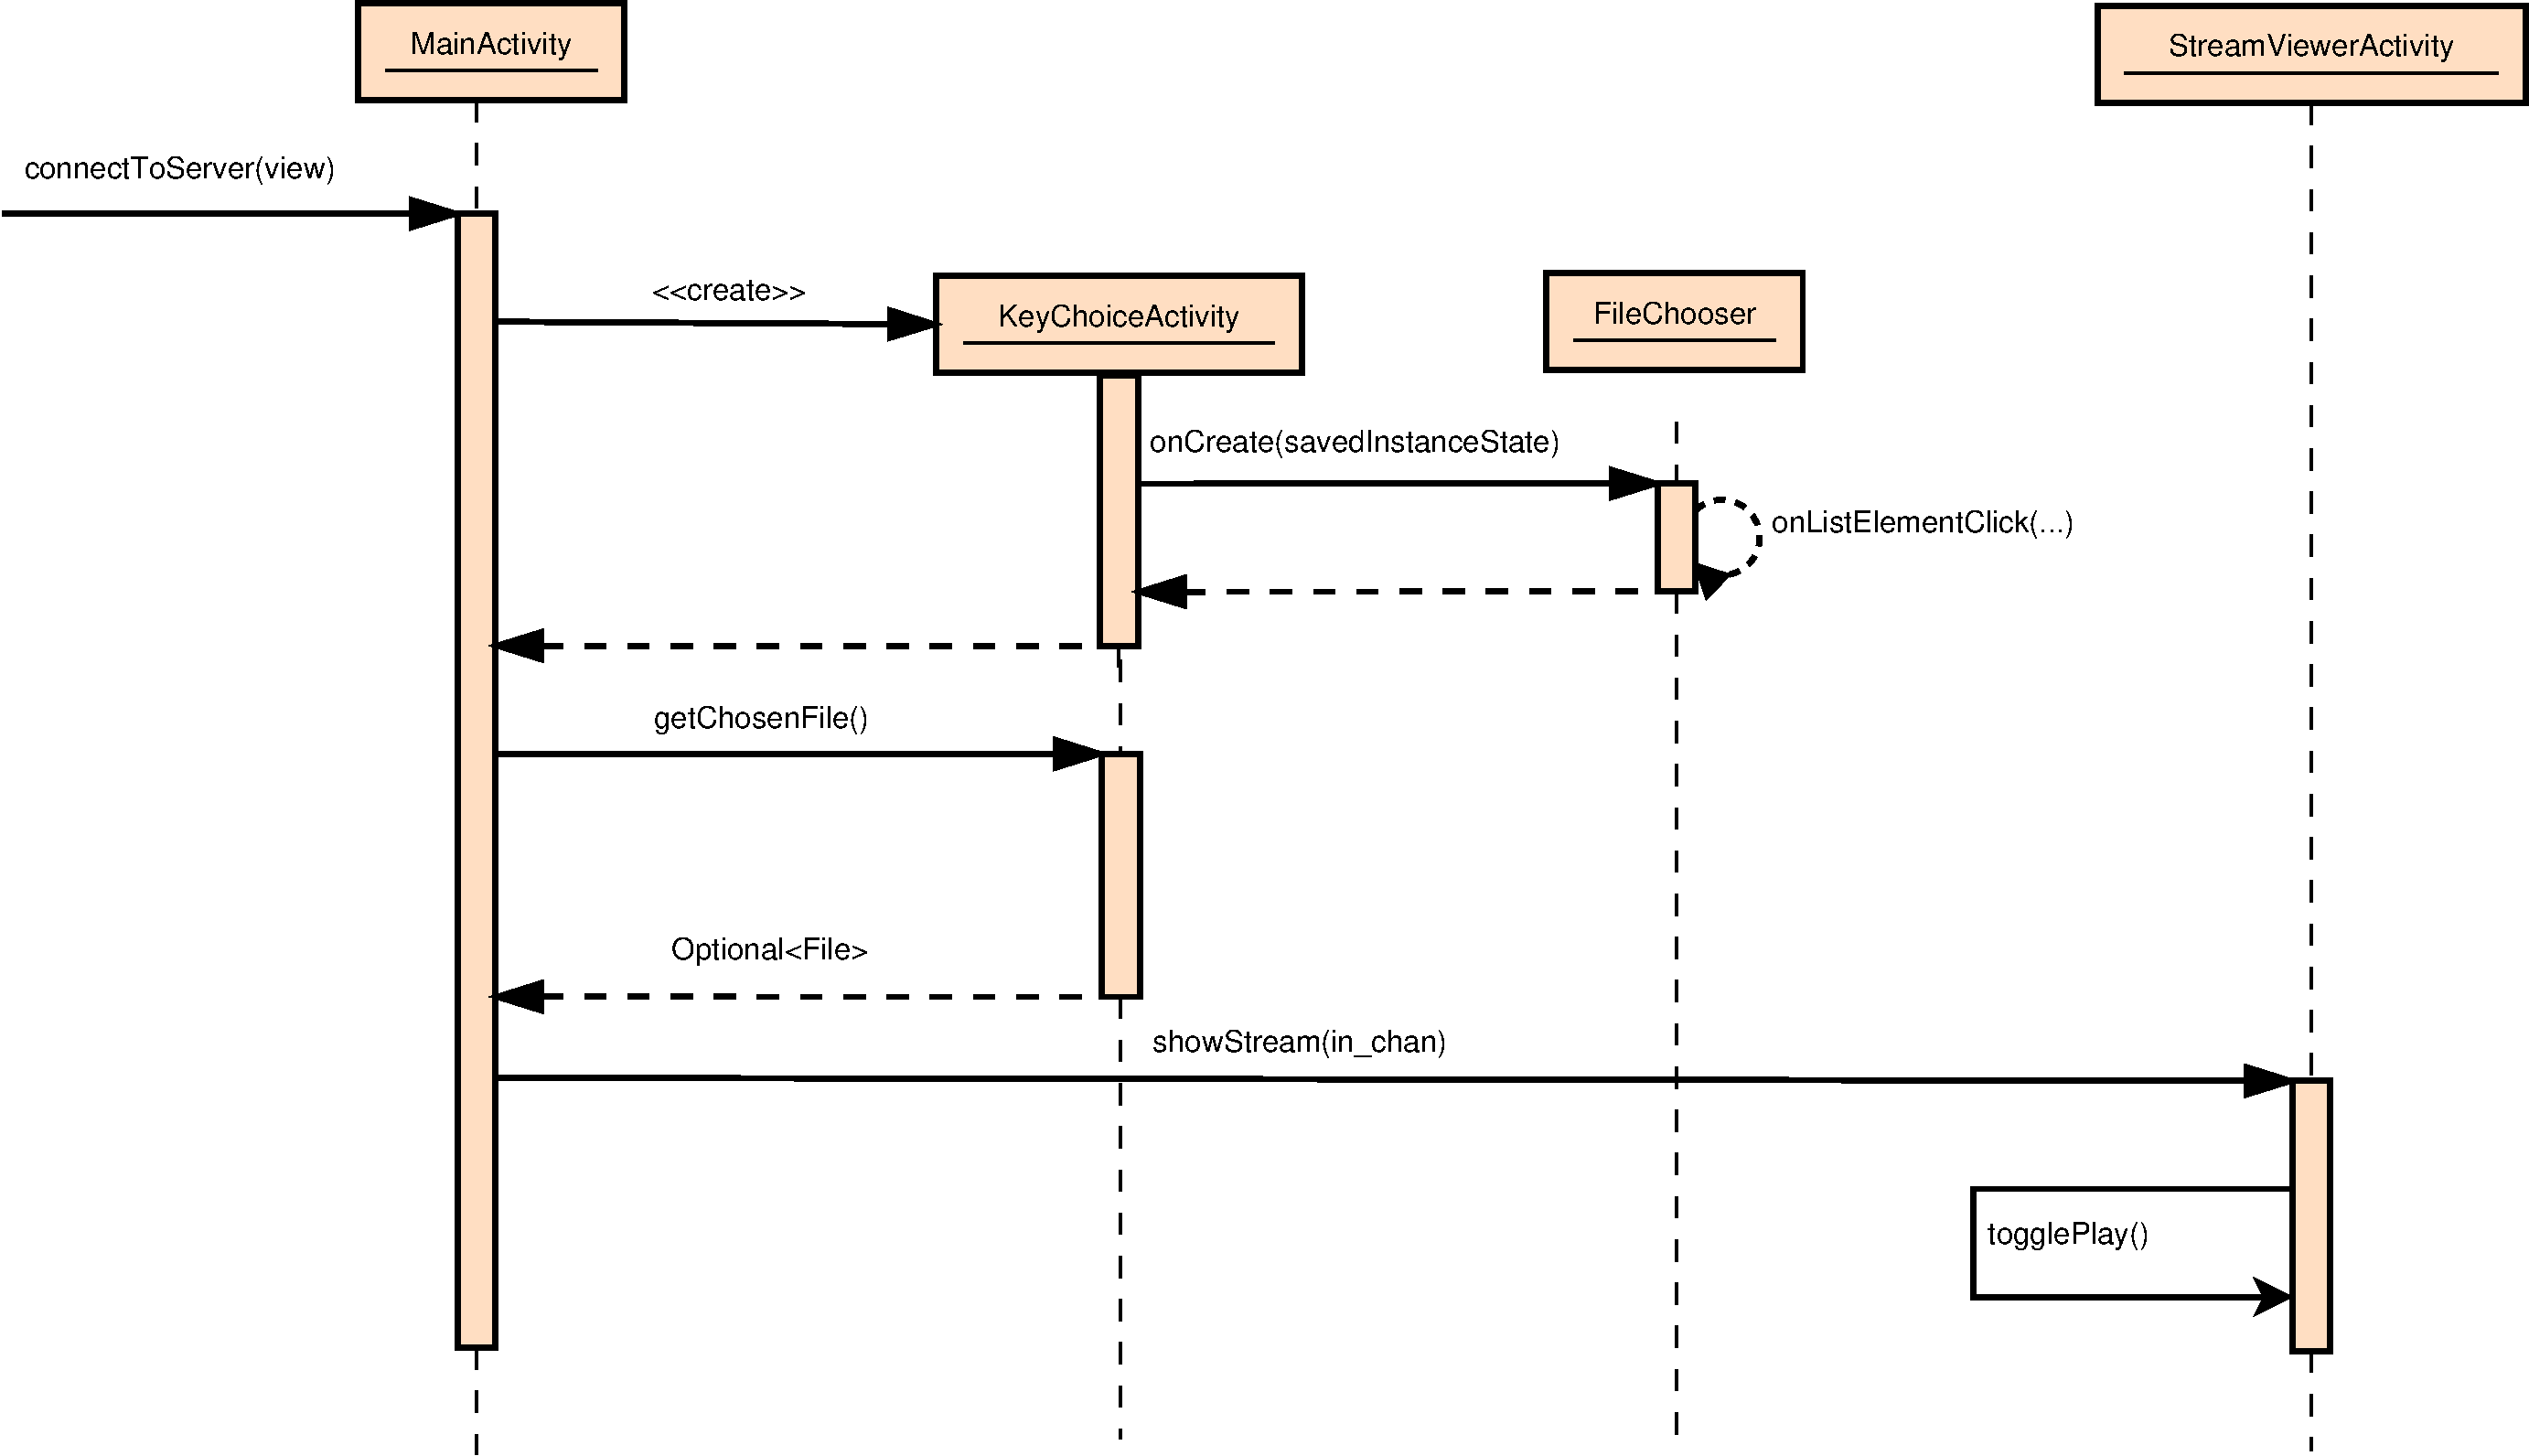
\includegraphics [width=400px] {figures/sequence_diagram_client/sequence_client.pdf}
\end{illustration}

\begin{landscape}
\begin{illustration}{Server: Passing a piece of plaintext data through to the client sockets.}
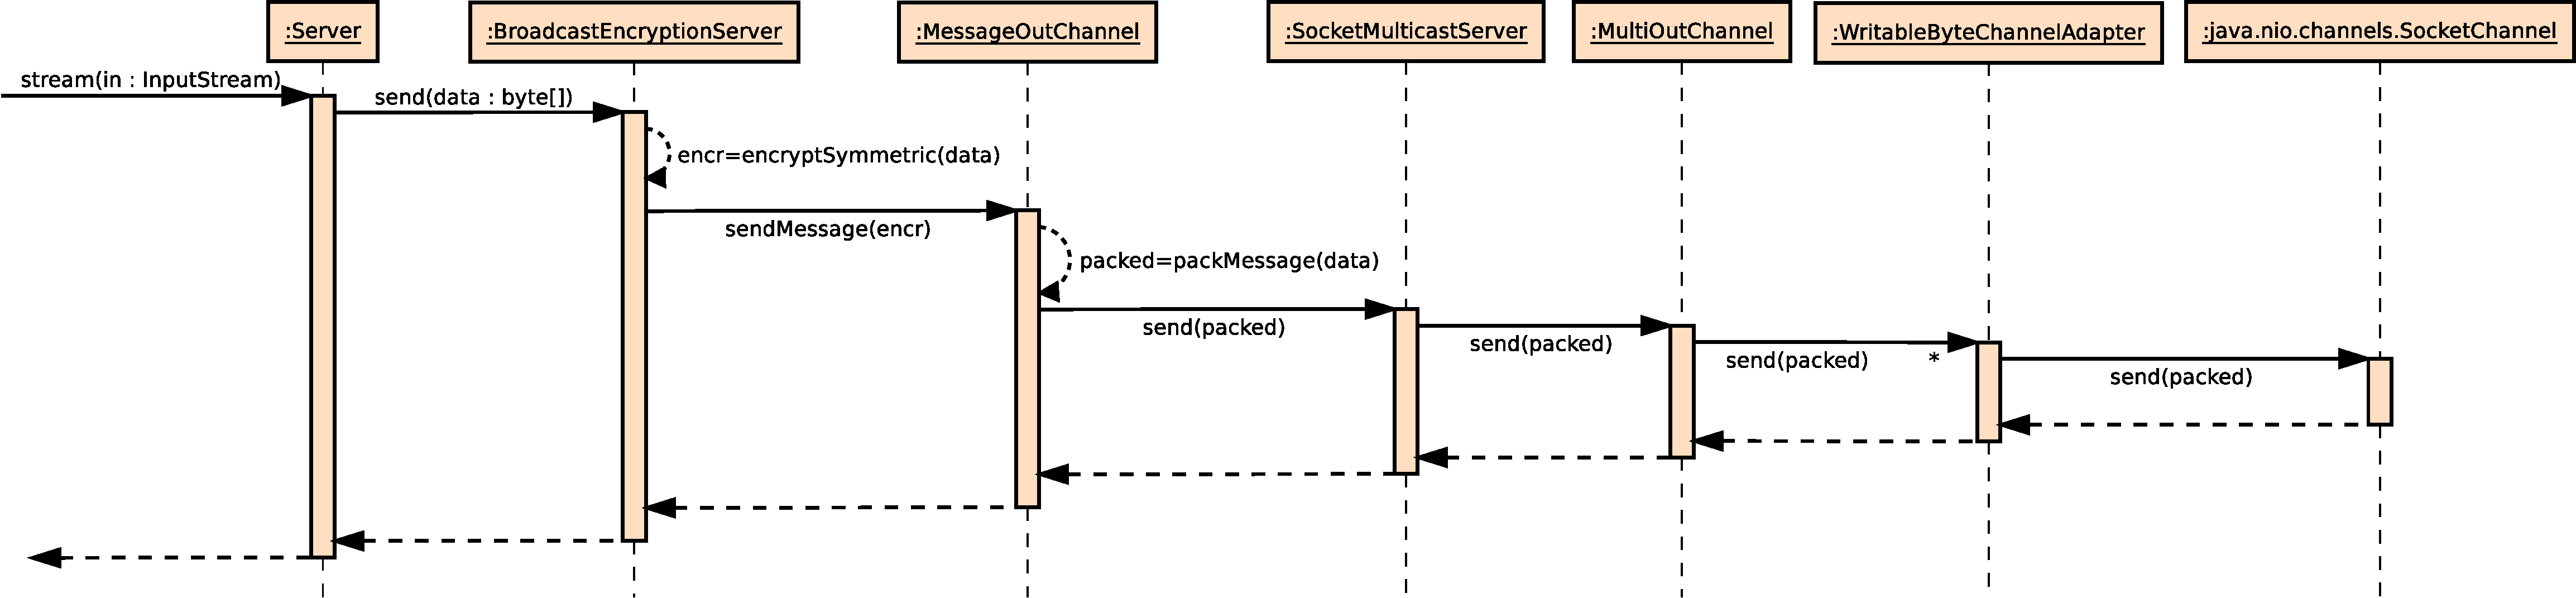
\includegraphics [width=700px] {figures/sequence_diagram_comm1_server/output.pdf}
\end{illustration}
\end{landscape}

\section{GUI design}
The interface should be user-friendly and intuitive to use. Therefore its design is kept minimalistic, focusing
on the main functionality and avoiding intrusive elements like an overuse of buttons.

\subsection{GUI visual examples}
The following images show prototypes of the client user interface.

\begin{illustration}{The main screen shown on startup.}
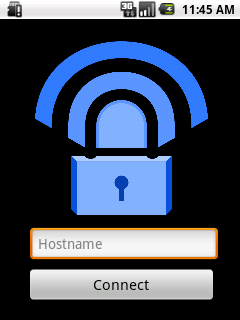
\includegraphics[width=150px]{figures/images/mainscreen.png}
\end{illustration}
\begin{illustration}{The menu popping up after the menu button is pressed.
   It allows navigation between the different screens.}
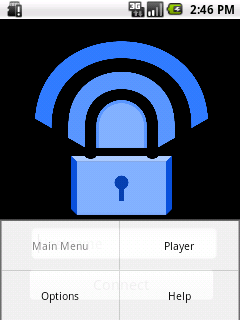
\includegraphics[width=150px]{figures/images/menu.png}
\end{illustration}
\begin{illustration}{The option screen which contains preferences, traffic statistics and a server history.}
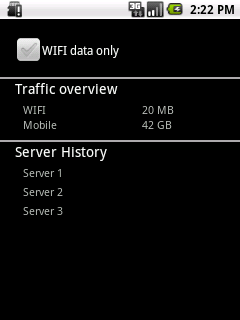
\includegraphics[width=150px]{figures/images/optionscreen.png}
\end{illustration}
\begin{illustration}{An example of an error message.}
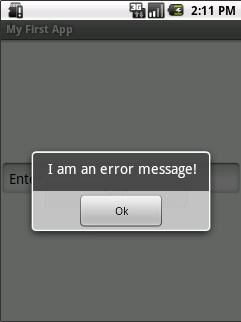
\includegraphics[width=150px]{figures/images/error.png}
\end{illustration}
\begin{illustration}{The file chooser to enable the user to select a private key.}
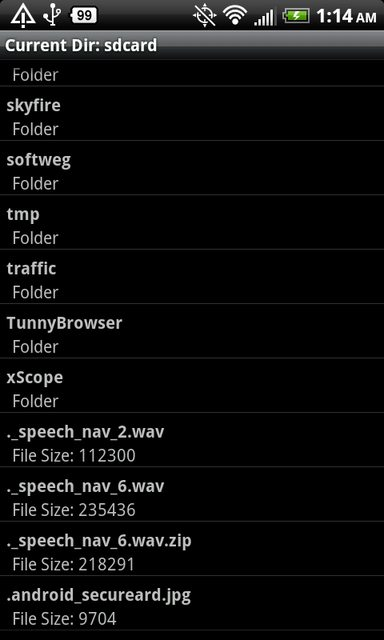
\includegraphics[width=150px]{figures/images/fileChooser.png}
\end{illustration}

\subsection{GUI activity}
\begin{illustration}{Activity diagram showing possible interactions with the client application.}
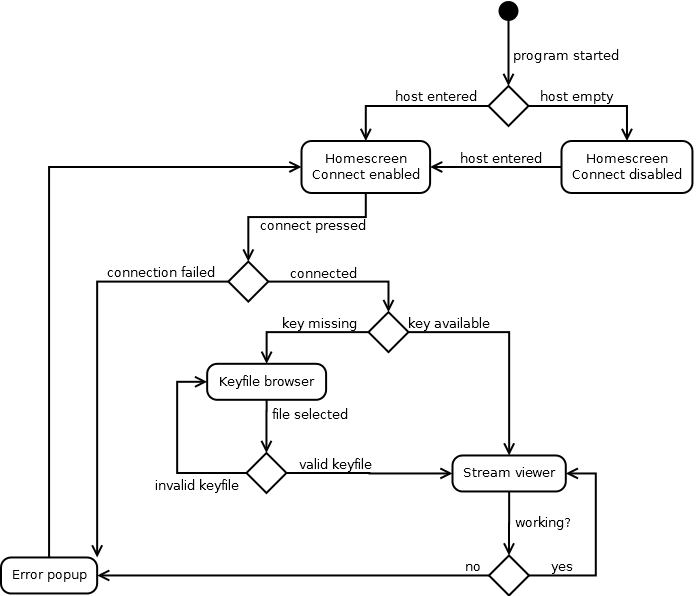
\includegraphics [width=500px]{figures/gui_activity_1/gui_activity_1.png}
\end{illustration}

\section{Time plan}
   \begin{illustration}{A rough time table for the implementation phase.}
  \begin{gantt}[xunitlength=0.5cm,fontsize=\small,titlefontsize=\small,drawledgerline=true]{9}{23}
    \begin{ganttitle}
      \titleelement{KW 51}{7}
      \titleelement{KW 2}{7}
      \titleelement{KW 3}{7}
       \titleelement{KW 4}{2}
    \end{ganttitle}
    \begin{ganttitle}
      \numtitle{17}{1}{23}{1}
      \numtitle{7}{1}{22}{1}
    \end{ganttitle}
    \ganttbar[color=yellow]{communication}{0}{3}
    \ganttbar[color=green]{cryptography}{3}{19}
    \ganttbar[color=blue]{server model}{3}{8}
    \ganttbar[color=blue]{server shell}{11}{11}
    \ganttbar[color=red]{client model}{3}{10}
    \ganttbar[color=red]{client view}{13}{9}
    \ganttbar{connect packages}{22}{1}

    \ganttcon{11}{4}{11}{5}
    \ganttcon{13}{6}{13}{7}

    \ganttcon{3}{2}{3}{3}
    \ganttcon{3}{2}{3}{4}
    \ganttcon{3}{2}{3}{6}
    \ganttcon{22}{3}{22}{8}
    \ganttcon{22}{5}{22}{8}
    \ganttcon{22}{7}{22}{8}
  \end{gantt}
  \end{illustration}

\bibliography{../bibtex/references}{}
\bibliographystyle{plain}

\end{document}

